\documentclass[10pt, a4paper, italian]{article}
\usepackage[T1]{fontenc}
\usepackage[utf8]{inputenc}
\usepackage{amsmath, amssymb, amsthm, thmtools, amsfonts, mathtools}
\usepackage{nicefrac}
\usepackage{calc}
\usepackage[pdftex, hyperindex, plainpages=false]{hyperref}
\usepackage[nameinlink]{cleveref} %load before classicthesis (clash)
%\usepackage[nochapters,pdfspacing]{classicthesis}
\usepackage{siunitx}
\usepackage[siunitx]{circuitikz}

\usepackage[a4paper]{geometry}
\usepackage{float}
\usepackage{mdframed}
\usepackage{titling}
\usepackage{booktabs}
\usepackage{graphicx}
\usepackage{caption, subcaption}
\usepackage{xcolor}
\usepackage[italian]{babel}
\usepackage{pgfplots}
\usepackage{listings}
%\usepackage{lmodern}
\usepackage{url}
\usepackage{enumitem}
\usepackage{tikz} %loads after classicthesis (xcolor incompat)

% lets graphicx know path where figures to be included are found
\graphicspath{{../figs/}}
\makeatletter
\def\input@path{{../figs/}}
%or: \def\input@path{{/path/to/folder/}{/path/to/other/folder/}}
\makeatother

% tikz pgf plots setup
\usepgfplotslibrary{external}
\pgfplotsset{compat=1.15}
%\tikzexternalize

% spaces and significant digits/figures for measurements
\sisetup{free-standing-units, space-before-unit, number-unit-product = \;,
scientific-notation = false, round-mode = figures, round-precision = 1,}

% turns all (hyperlinked) references black [default is blue]
\hypersetup{
	linktoc=all,
	colorlinks=true,
	linkcolor=black
}

% code listings config
%\lstset{
%language=Python,
%basicstyle=\ttfamily,
%columns=fullflexible,
%keepspaces=true,
%}

% mdframed (for boxed text) configuration
\mdfsetup{linewidth=0.6pt}

% Default fixed font does not support bold face
\DeclareFixedFont{\ttb}{T1}{txtt}{bx}{n}{12} % for bold
\DeclareFixedFont{\ttm}{T1}{txtt}{m}{n}{12}  % for normal

% Custom colors
\usepackage{color}
\definecolor{deepblue}{rgb}{0,0,0.5}
\definecolor{deepred}{rgb}{0.6,0,0}
\definecolor{deepgreen}{rgb}{0,0.5,0}

% Commands 
\newcommand{\executeiffilenewer}[3]{%
	\ifnum\pdfstrcmp{\pdffilemoddate{#1}}%
		{\pdffilemoddate{#2}}>0%
	{\immediate\write18{#3}}\fi%
}
% input .svg --> .pdf_tex graphs
%\newcommand{\includesvg}[1]{%
%	\executeiffilenewer{#1.svg}{#1.pdf}%
%	{inkscape -z -D --file=#1.svg %
%	--export-pdf=#1.pdf --export-latex}%
%	\input{#1.pdf_tex}%
%}
% Thanks UniPi's Department of Physics E. Fermi
\newcommand{\thanksdf}{(\thanks{Dipartimento di Fisica E.~Fermi,%
Universit\`a di Pisa - Pisa, Italy.}\;)}

% hyperlink to email address
\newcommand{\mail}[1]{\href{mailto:#1}{\textsf{#1}}}

% \vec for bold vectors, instead of overarrows (now "\arrvec")
\let\arrvec=\vec
\renewcommand{\vec}[1]{\boldsymbol #1}
% replaces straight phi with slanted phi
\renewcommand{\phi}{\varphi}
% replaces straight eps with curved epsilon
\newcommand{\eps}{\varepsilon}
% abbreviation for (sub_/super^)scripts of \lim, \sum,... in inline math
\newcommand{\ds}{\displaystyle}

% blackboard/number set letters
\newcommand{\CC}{\mathbb C}
\newcommand{\HH}{\mathbb H}
\newcommand{\KK}{\mathbb K}
\newcommand{\NN}{\mathbb N}
\newcommand{\PP}{\mathbb P}
\newcommand{\QQ}{\mathbb Q}
\newcommand{\RR}{\mathbb R}
\newcommand{\ZZ}{\mathbb Z}

\newcommand{\Abs}[1]{{\left\Vert #1\right\Vert}}
\newcommand{\enclose}[1]{{\left( #1 \right)}}
\newcommand{\Enclose}[1]{{\left[ #1 \right]}}
\newcommand{\floor}[1]{\left\lfloor #1 \right\rfloor}
\newcommand{\ceil}[1]{\left\lceil #1 \right\rceil}
\newcommand{\To}{\rightrightarrows}

% Math operators
\DeclareMathOperator{\divergence}{div}
\renewcommand{\div}{\divergence}
\DeclareMathOperator{\Imaginarypart}{Im}
\renewcommand{\Im}{\Imaginarypart}
\DeclareMathOperator{\Realpart}{Re}
\renewcommand{\Re}{\Realpart}
%\DeclareMathOperator{\arg}{arg}
\DeclareMathOperator{\tg}{tg}
\DeclareMathOperator{\arctg}{arctg}
\DeclareMathOperator{\settsinh}{settsinh}
\DeclareMathOperator{\settcosh}{settcosh}
\DeclareMathOperator{\tr}{tr}
\DeclareMathOperator{\im}{im}
\DeclareMathOperator{\sgn}{sgn}
\DeclareMathOperator{\diag}{diag}

\DeclarePairedDelimiter{\norm}{\lVert}{\rVert}
\DeclarePairedDelimiter{\scalar}{\langle}{\rangle}

% Logarithm with arbitrary base.
% -> log_10
\newcommand{\llog}[1][10]{\log_{#1}}

% Absolute value.
% -> |x|
\newcommand{\abs}[1]{\left| #1 \right|}

% Powers.
% -> x^a
\newcommand{\power}[2][2]{\left( #2 \right)^{#1}}

% Square.
% -> x^2
\newcommand{\sq}[1]{\power[2]{#1}}

% Expansion of the binomial coefficient.
% -> n1!/(n2!(n1 - n2)!)
\newcommand{\binomexpr}[2]{\frac{#1!}{#2!(#1 - #2)!}}

% Expression evaluation at a given point with square brackets.
% -> [x]_{a}
\newcommand{\at}[2]{\left[ #1\right]_{\makebox[-1pt][l]{${\scriptstyle#2}$}}}

% Expression evaluation in an interval.
% -> [x] _{a}^{b}
\newcommand{\eval}[3]{\left.#1%
  \right|_{\makebox[-1pt][l]{${\scriptstyle#2}$}}^{\makebox[-1pt][l]{${\scriptstyle#3}$}}}

% Upright d in math mode (for differentials).
% -> d
\newcommand{\ud}{\mathrm{d}}

% Differential.
% -> dx
\newcommand{\diff}[1][x]{\,\ud{#1}}

% Base command for defining derivatives.
% -> df/dx or d^kf/dx^k
\newcommand{\basederivative}[4][]{%
  \displaystyle%
  \ifx\\#1\\\frac{#4#2}{#4#3}%
  \else%
  \frac{#4^#1#2}{#4#3^#1}%
  \fi%
}

% Total derivative.
% -> df/dx(x) or d^kf/dx^k(x)
\newcommand{\td}[4][]{%
  \basederivative[#1]{#2}{#3}{\ud}%
  \ifx\\#4\\%
  \else%
  \mkern-4mu\left(#4\right)%
  \fi%
}

% Partial derivative.
% -> df/dx(x) or d^kf/dx^k(x)
\newcommand{\pd}[4][]{%
  \basederivative[#1]{#2}{#3}{\partial}%
  \ifx\\#4\\%
  \else%
  \mkern-4mu\left(#4\right)%
  \fi%
}

\newcommand{\intinf}{\int_{-\infty}^{\infty}\!\!\!}

\newcommand{\cinterval}[2]{\left[\, #1,~#2 \,\right]}

\newcommand{\linterval}[2]{\left[\, #1,~#2 \,\right)}

\newcommand{\rinterval}[2]{\left(\, #1,~#2 \,\right]}

\newcommand{\ointerval}[2]{\left(\, #1,~#2 \,\right)}

\newcommand{\prob}[1]{\displaystyle P\left(#1\right)}

\newcommand{\pvalue}{\emph{$p$-value}}

\newcommand{\cond}{\,|\,}

\newcommand{\expect}[1]{\displaystyle E\left[#1\right]}

\newcommand{\mom}[2][]{\displaystyle {\cal M}_{#2}\ifx\\#1\\\else(#1)\fi}

\newcommand{\momalg}[1]{\displaystyle \lambda_{#1}}

\newcommand{\momcen}[1]{\displaystyle \mu_{#1}}

\newcommand{\skewness}{\displaystyle \gamma_1}

\newcommand{\kurtosis}{\displaystyle \gamma_2}

\newcommand{\charf}[1][x]{\phi_{#1}}

\newcommand{\momgenf}[1][x]{M_{#1}}

\newcommand{\fwhm}{{\scriptstyle \textsc{FWHM}}}

\newcommand{\hwhm}{{\scriptstyle \textsc{HWHM}}}

\newcommand{\median}{\mu_{\nicefrac{1}{2}}}

\newcommand{\var}[1]{\ensuremath{\text{Var}\left(#1\right)}}

\newcommand{\cov}[2]{\ensuremath{\text{Cov}\left(#1, #2\right)}}

\newcommand{\corr}[2]{\ensuremath{\text{Corr}\left(#1, #2\right)}}

\newcommand{\like}{\mathcal L}

\newcommand{\likelihood}[2][]{\like\ifx\\#2\\\else(#2\ifx\\#1\\\else;#1\fi)\fi}

\newcommand{\chisq}{\ensuremath{\chi^2}}

\newcommand{\chisquare}[2][]{\chisq\ifx\\#2\\\else(#2\ifx\\#1\\\else;#1\fi)\fi}

\newcommand{\loglikelihood}[2][]{\log\likelihood[#1]{#2}}

\newcommand{\pdf}[3][]{#2(#3\ifx\\#1\\\else;#1\fi)}

\newcommand{\binomialpdf}[2][]{\pdf[#1]{\mathcal B}{#2}}

\newcommand{\multinomialpdf}[2][]{\pdf[#1]{\mathcal M}{#2}}

\newcommand{\poissonpdf}[2][]{\pdf[#1]{\mathcal P}{#2}}

\newcommand{\uniformpdf}[2][]{\pdf[#1]{u}{#2}}

\newcommand{\exponentialpdf}[2][]{\pdf[#1]{\varepsilon}{#2}}

\newcommand{\gausspdf}[2][]{\pdf[#1]{N}{#2}}

\newcommand{\chisquarepdf}[2][]{\pdf[#1]{\wp}{#2}}

\newcommand{\cauchypdf}[2][]{\pdf[#1]{c}{#2}}

\newcommand{\erf}[1]{\ensuremath{\text{erf}\left(#1\right)}}

\newcommand{\dccases}[4][]{#2 \ifx\\#2\\\else=\fi %
  \begin{cases}
    \displaystyle #3 & \text{per variabili discrete}\\
    \displaystyle #4 & \text{per variabili continue}#1
  \end{cases}
}
% sub/super-scriptable for all symbol as math operator 
\newcommand\Scaleforall[1]{\vcenter{\hbox{\scalefont{#1}$\forall$}}}

\DeclareMathOperator*\forevery{%
  \vphantom\sum
  \mathchoice{\Scaleforall{2}}{\Scaleforall{1.4}}{\Scaleforall{1}}{\Scaleforall{0.75}}}
\geometry{left=2cm, right=2cm, top=2cm, bottom=2cm}

% indexes subsections with letters, sections with numbers (1.a, 1.b, ...)
\renewcommand{\thesubsection}{\thesection.\alph{subsection}}

% lets graphicx know path where figures to be included are found
\graphicspath{{../figs/}}

\author{Gruppo 1.AC \\ Matteo Rossi, Bernardo Tomelleri}
\title{Es11: Esperimenti di Interferometria per misure di lunghezze d'onda}
\begin{document}
\date{\today}
\maketitle

%=======================
\section{Scopo dell'esperienza}
Lo scopo dell'esperienza è misurare la lunghezza d'onda di un laser
a semiconduttore studiando il pattern di diffrazione generato da un suo
fascio incidente sulla scala millimetrata di un calibro.

\section{Descrizione della misura}
Per la misura si utilizza il righello graduato di un calibro come reticolo di diffrazione in riflessione con passo reticolare $ d = \SI{1}{\milli\meter} $.  Si fa incidere, ad angolo radente, un fascio laser sul reticolo, questo produce su uno schermo posto a distanza $ D $ una serie di ordini di diffrazione indicizzati con la lettera $m \in \ZZ$, come è illustrato in Figura~\ref{fig:schema}. I massimi di diffrazione si hanno in corrispondenza degli spot del laser sullo schermo e sono individuati dagli angoli $\theta_{\mathrm{d},m}$ in figura.

Nell'esperienza gli angoli $\theta_{\mathrm{d},m}$ si ricavano dagli angoli $\alpha_m = \pi/2 - \theta_{\mathrm{d},m}$ rispetto all'orizzontale, questi ultimi ottenuti dalla misura sperimentale delle altezze $h_m = D \tan\alpha_m$ del centro di ogni spot rispetto allo zero dell'asse verticale che corrisponde alla quota del calibro.

L'equazione del reticolo che lega la posizione dei massimi di diffrazione alla lunghezza d'onda $\lambda$ della luce incidente e al passo reticolare $d$ è:
\begin{equation}\label{eq:fit}
    m \lambda = d \left(\sin{\theta\ped{i}} - \sin{\theta_{\mathrm{d},m}}\right).
\end{equation}

La relazione che lega la lunghezza d'onda all'angolo di riflessione $\theta_m$ è:
\[
{\sin{\theta_m}=sin{\theta_i}-\frac{m\lambda}{d}}{theta}
\]
dove $d=\SI{1}{\milli \meter}$ è il passo reticolare e $\theta_i$ l'angolo di riflessione. L'angolo di incidenza si ricava dalle altezze misurate sulla carta millimetrata $h_m$ rispetto alla baseline (altezza del calibro) con:
\[
{\sin{\theta_m}=\left[ 1+\left(\frac{h_m}{D}\right)^2\right]^{-\frac{1}{2}}}
\]
dove $D$ è la distanza dal centro dello spot di luce sul calibro al muro. Poichè l'incidenza del laser è quasi radente lo spot sul calibro è allungato, per misurarlo è stato utilizzato il centro dello spot come valore di misura e la semilarghezza come errore, la media pesata delle misure dei componenti del gruppo da 
\[
{D= \SI{304.3 \pm 1.7}{\centi \meter}}
\]
Mentre la baseline stimata come media tra l'ordine 0 di interferenza (riflessione pura) e il fascio non diffratto è (per ogni componente del gruppo):
\[
\begin{array}{lccc}
\toprule
\mathrm{Componente} & 1& 2 &3 \\
\midrule
BL \; \si{\centi \meter}&18.0 & 18.3 &18.0 \\
\sigma(BL)\; \si{\centi \meter}& 0.4&  0.4 & 0.5\\
\bottomrule
\end{array}
\]
Per quanto riguarda le altezze, bisogna considerare che gli spot sulla carta millimetrata sono allungati, per tenerne conto è stato considerato un errore circa pari alla semilarghezza degli spot di luce sulla carta millimetrata, sommato in quadratura all'errore di lettura del valore centrale rispetto alla carta millimetrata. Dopo di che è stata sottratta la baseline sommando in quadratura gli errori. \newline
In tabella \ref{hm} sono riportate le medie pesate dei dati di ogni componente del gruppo, e dunque il valore corrispondente di $\sin{\theta_m}$ e il corrispondente errore:
\[
\begin{array}{ccccc}
\toprule
m & h_m \; (\si{\centi \meter}) & \sigma(h_m) \; (\si{\centi \meter}) & \sin{\theta_m} & \sigma(\sin{\theta_m}) \\
\midrule
0&7.6     & 0.4 & 0.99970  & 0.00004 \\
1&13.4    & 0.4 & 0.99905  &  0.00006 \\
2&17.2    & 0.4 & 0.99842  &  0.00007\\
3&20.3    & 0.4&  0.9977  & 0.0001   \\
4&23.2    & 0.4&  0.9971 & 0.0001\\
5&25.5    & 0.3 & 0.9964 & 0.0001\\
6&27.9    & 0.3 & 0.99579 &0.00013\\
7&29.9    & 0.3 & 0.99516 & 0.00014 \\
8&31.9    & 0.3 & 0.99455 &0.00015\\
9&33.6    & 0.3 & 0.99393 &0.00016\\
10&35.5   & 0.3 & 0.99327 &0.00017\\
11&37.2   & 0.3& 0.9926  &0.0002 \\
12&38.8   & 0.3& 0.9920  & 0.0002\\
13&40.2   & 0.3& 0.9914 & 0.0002\\
14&41.7   & 0.3& 0.9907 & 0.0002 \\
15&43.3   & 0.3& 0.9900  &0.0002 \\
16&44.6  &  0.3& 0.9894  & 0.0002\\
17&45.8  &  0.3& 0.9888   &0.0002\\
18&47.2  &  0.3 & 0.9882  & 0.0002\\
19&48.4  &  0.3  & 0.9875  & 0.0002\\
20&49.6   &  0.3   &0.9869   & 0.0002\\ 
21&50.9   & 0.3    & 0.9863  &0.0003 \\
22&52.0   &  0.3 & 0.9857 & 0.0003\\
\bottomrule
\end{array}
\]
\captionof{table}{Tabella dei dati di altezze e angoli (media pesata). \label{hm}}
\vspace{0.2cm}
A questo punto tramite un fit lineare $\sin{\theta_m}$ vs $m$ partendo dall'equazione \eqref{theta} è possibile stimare il parametro $\frac{\lambda}{d}$ e dunque $\lambda$. Nell'effettuare il fit è stato tenuto conto che la maggior parte degli errori è di tipo sistematico (incertezza su D, data dal metro a nastro e dalla posizione dello spot, e dalla posizione degli spot su carta millimetrata rispetto alla loro estensione) ed è stato utilizzato il flag absolute\textunderscore sigma=True in modo che la funzione curve\textunderscore fit non riscalasse gli errori dati in input. \newline
Il grafico della retta di best fit e dei residui è riportato in figura \ref{fit}
\begin{center}
%   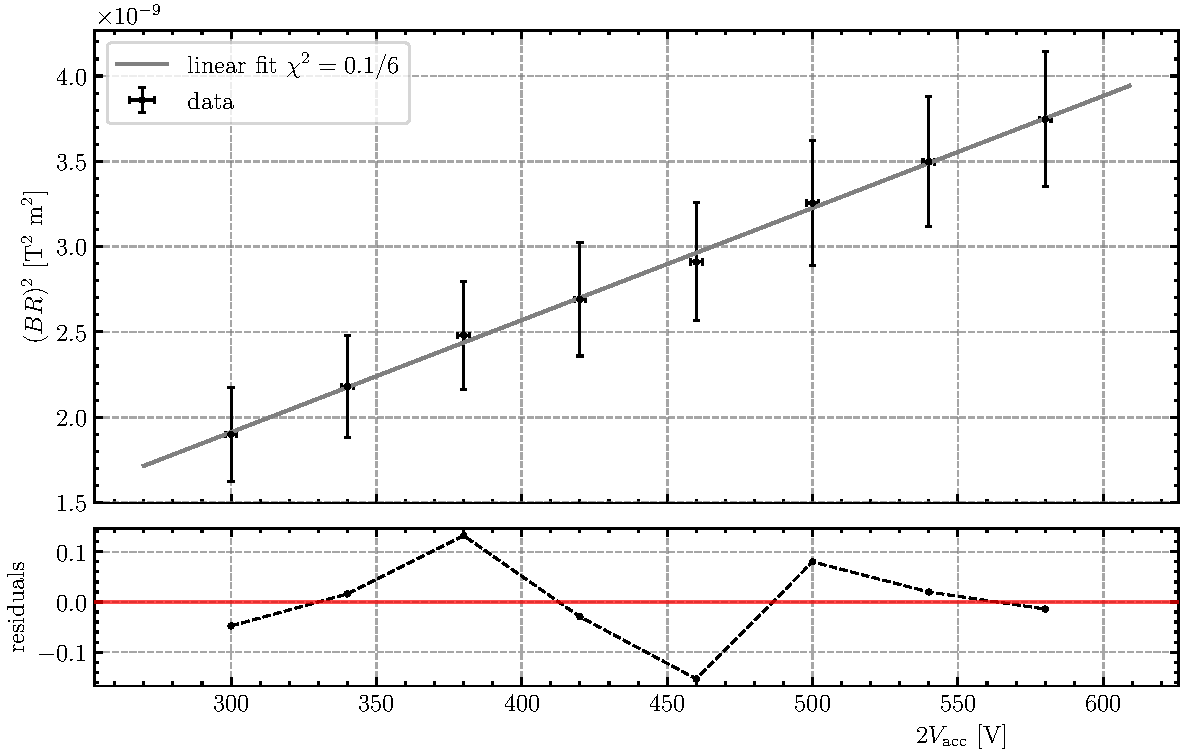
\includegraphics[width=\textwidth]{lin}
    \captionof{figure}{Retta di best fit e grafico dei residui \label{fit}}
\end{center}
I parametri stimati sono:

\[
{\lambda= \SI{639 \pm 4}{\nano \meter} \;\; \chi^2 /\mathrm{dof}=0.80/21}
\]
Compatibile con il valore indicato sul datasheet del laser: $\lambda=\SI{636\pm1}{\nano \meter}$

%=======================
\section{Interferometro di Michelson: lunghezza d'onda lampada Hg}
\subsection{Stima del fattore di conversione della vite}
Per stimare il fattore di conversione tra lo spostamento del nonio della vite e lo spostamento dello specchio mobile M1 del Michelson, è stato utilizzato un laser He-Ne a lunghezza d'onda nota $\lambda= \SI{632.8}{\nano \meter}$\footnote{L'incertezza, in genere $<\SI{1}{\nano \meter}$ per laser a HeNe, dunque dell'ordine di alcune parti per mille, è stata trascurata in quanto si vedrà in seguito che gli errori su $\eta$ dati dagli altri parametri sono molto più significativi}. Da cui tramite la relazione tra il numero di frange contate ($m$) e lo spostamento del braccio ($\Delta L$) (equazione che definisce il funzionamento del Michelson)
\[
{\Delta L=\frac{m \lambda}{2}}{michelson}
\]
si ricava il fattore $\eta$:
\[
\eta=\frac{\Delta L}{\Delta L'}= \frac{m \lambda}{2 \Delta L'}
\]
Con $\Delta L'$ spostamento della vite. \newline
\subsubsection*{$L'\simeq \SI{0}{\micro \meter}$}
Nella seguente tabella si riportano i valori delle frange contate e degli spostamenti della vite misurati dai diversi componenti del gruppo. L'errore sulle frange è dovuto al fatto che durante la misura la vite in alcuni momenti scorreva nel verso opposto rendendo difficile contare le frange correttamente, anche con il video rallentato. La presa dati è stata spezzata in due parti (dette a e b) in modo da verificare la consistenza dei parametri trovati ed è indicata nella colonna a sinistra. I separatori individuano le misure dei diversi componenti del gruppo.

A questo punto è possibile calcolare i fattori eta in ciascuna delle due parti delle prese dati e quello considerando invece lo spostamento complessivo, facendo una media pesata delle misure di $m $ e $\Delta L'$ presi dai componenti del gruppo si trova
\[
\def\arraystretch{1.5}
\begin{array}{rcl}
\eta_{1a} & = & 1.97\pm 0.14\\
\eta_{1b} & = & 1.45\pm 0.11\\
\eta_{1}&=&1.67 \pm 0.09
\end{array}
\]

Conoscendo il fattore di proporzionalità tra $\Delta L$ e $ \Delta L'$ è possibile ora stimare la $\lambda_{Hg}$ dalla stessa relazione \eqref{michelson}:
\[
{\lambda=\frac{2 \Delta L}{m}=\frac{2\eta \Delta L'}{m}}
\]
Utilizzando la media pesata di $\eta$ nelle zone 1 e 2 si ottiene:
\[
{\lambda=\SI{607\pm62}{\nano \meter}}
\]
Questo valore è compatibile con il valore atteso ($\SI{546}{\nano \meter}$).\newline
Come accennato nella sezione precedente, si potrebbe ipotizzare (a posteriori) che il funzionamento della vite nella zona 1 abbia dei problemi, e dunque scartare questo valore di $\eta$, utilizzando per il calcolo di $\lambda_{Hg}$ il solo valore $\eta_2$ si ottiene:
\[
{\lambda=\SI{549\pm54}{\nano \meter}}
\]
Valore compatibile con quanto atteso e con un valore centrale più vicino al valore atteso.

%=======================
\section*{Conclusioni e commenti finali}
In quest'esperienza è stato possibile determinare con successo la lunghezza d'onda di un laser a semiconduttore utilizzando un calibro come reticolo di diffrazione. Inoltre, utilizzando un interferometro di Michelson è stata stimata la lunghezza d'onda della riga verde di una lampada a mercurio. Nonostante alcune difficoltà incontrate in quest'ultima stima e le sorgenti di errore abbastanza rilevanti, è stato possibile ottenere una stima compatibile con il valore atteso.

%=======================
\section*{Dichiarazione}
I firmatari di questa relazione dichiarano che il contenuto della relazione \`e
originale, con misure effettuate dai membri del gruppo, e che tutti i firmatari
hanno contribuito alla elaborazione della relazione stessa.


\end{document}
